\documentclass[border=0mm]{standalone}

\usepackage{import}
\subimport{../../../}{preamble.tex}

\usepackage{tikz}
\usetikzlibrary{calc}
\usepackage{pgfplots}

\begin{document}

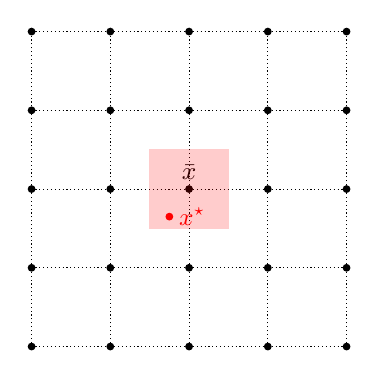
\begin{tikzpicture}

  \foreach \x in {0,1,...,4}
  {
    \foreach \y in {0,1,...,4}
    {
      \node[circle,inner sep=1,fill=black] at (\x, \y) {};
    }
  }

  \foreach \x in {0,1,...,3}
  {
    \foreach \y in {0,1,...,3}
    {
      \draw[densely dotted] (\x, \y) -- (\x+1, \y) {};
      \draw[densely dotted] (\x, \y) -- (\x, \y+1) {};
    }
  }

  \foreach \x in {4}
  {
    \foreach \y in {0,1,...,3}
    {
      \draw[densely dotted] (\x, \y) -- (\x, \y+1) {};
    }
  }

  \foreach \x in {0,1,...,3}
  {
    \foreach \y in {4}
    {
      \draw[densely dotted] (\x, \y) -- (\x+1, \y) {};
    }
  }
  
  \node[above] (xbar) at (2, 2) {\small $\bar x$};
  \draw[draw=red, fill=red, opacity=0.2] (1.5,2.5) rectangle (2.5,1.5);

  \node[circle,inner sep=1,fill=red] (xstar) at (1.75, 1.65) {};
  \node[right, red] at (xstar) {\small $x^\star$};
\end{tikzpicture}

\end{document}

%%% Local Variables:
%%% mode: latex
%%% TeX-master: t
%%% End:
